% Generated from: Zhihu/专栏：概率与统计/渐近统计 (7)：极大似然估计_金鱼马_2026-05-08.md
\section{基本概念}

\subsection{似然函数与最大似然估计}

首先简单回顾一下 MLE 的概念。设 $X_1,\dots,X_n$ 是独立同分布 (i.i.d.) 的随机变量，其分布 $P_\theta$ 属于参数族 $\mathscr P=\{P_\theta:\theta=(\theta_1,\dots,\theta_k)^\top\in\Theta\}$，参数空间 $\Theta\subset\mathbb R^k$ ；每个 $P_\theta$ 关于某 $\sigma$ -有限的控制测度 $\mu$ 绝对连续，从而有密度 $p_\theta(x)=\tfrac{\mathrm dP_\theta}{\mathrm d\mu}(x)$。

在样本 $X=(X_1,\dots,X_n)$ 下，定义\textbf{\emph{似然函数}} (Likelihood function) 为
\[L_n(\theta) := \prod_{j=1}^n p_\theta(X_j)\]
这是一个关于 $\theta$ 的函数，相当于用样本的``果''来衡量真实参数的``因''。通常我们取其对数以将乘积化为求和，从而得到如下对数似然函数：
\[\ell_n(\theta):=\log L_n(\theta)=\sum_{j=1}^n\log p_\theta(X_j)\]
\textbf{\emph{极大似然估计}} $\widehat\theta$ 就是最大化该对数似然的参数值：
\[
\widehat\theta := \operatorname*{\arg\max}_{\theta\in\Theta}\ell_n(\theta).
\]

在似然函数可导的条件下，这等价于求解如下\textbf{\emph{对数似然方程}} ：
\[
\sum_{j=1}^n\frac{\partial\log p_\theta(X_j)}{\partial \theta_i}=0,\quad i=1,2,\dots,k.
\]

称对数似然函数的导数（梯度）为\textbf{\emph{得分函数}} (Score function)。

% 关于 MLE 的一些例子和讨论，可见

% \href{https://zhuanlan.zhihu.com/p/1906791960641007646}{数理统计 (14) : 极大似然估计 (MLE) - 上}

% \href{https://www.zhihu.com/question/24124998}{如何通俗地理解概率论中的「极大似然估计法」?}

我们这里主要讨论其渐近性质，即当样本量 $n\to\infty$ 的条件下，MLE $\widehat\theta$ 有多好？

\subsection{Fisher 信息}

参数族 $\mathscr P$ 的 Fisher 信息 (Fisher Information, FI) 衡量了分布随参数变化的``敏感度''------对数似然的陡峭程度；其值越大，似然函数越陡峭，数据就越容易区分不同的参数值。

\begin{definition*}[Fisher 信息正则性]
设参数族 $\mathscr{P}=\{P_\theta:\theta\in\Theta\}$ 被 $\sigma$-有限测度 $\mu$ 控制，对某 $\theta\in\Theta$，设

\begin{enumerate}
\def\labelenumi{\arabic{enumi}.}
\tightlist
\item
  存在 $\theta$ 的一个开邻域 $\Theta_0$，使得 $p_{\theta'}(x)>0$ 对所有 $x$ 和 $\theta'\in\Theta_0$ 成立；
\item
  对每个 $x$，$p_\theta(x)$ 在 $\theta$ 处可微；
\item
  等式 $\int p_\theta(x)\mathrm d\mu(x)=1$ 可在积分号下求导，即
\end{enumerate}
\[\int\frac{\partial}{\partial\theta}p_\theta(x)\mathrm d\mu(x)=0\]
那么称 $\mathscr P$ (在 $\theta$ 处) 是 \textbf{\emph{Fisher 信息正则}} (FI regular) 的。
\end{definition*}

\begin{definition*}[Fisher 信息]
设参数族 $\mathscr{P}=\{P_\theta:\theta\in\Theta\}$ 是 FI 正则的，其中 $\Theta\subset\mathbb R$，定义
\[
I(\theta)=\mathbb{E}_\theta\left[\left(\frac{\partial}{\partial\theta}\log p_\theta(X)\right)^2\right].
\]

为其在 $\theta$ 处的 Fisher 信息。
\end{definition*}

\begin{remark}

\begin{itemize}
\tightlist
\item
  当我们谈论 Fisher 信息时总假设其大于 0，否则 $I(\theta)=0$ 表明参数与分布是无关的。
\item
  这里的值 $X$ 可以视作从总体中抽取的单个样本；若是有 $n$ 个 i.i.d. 样本，它们的 Fisher 信息应为 $nI(\theta)$ 。
\item
  根据 FI 正则定义中的 (3.)，得分函数的期望为 0： $\mathbb E_\theta\left[\tfrac{\partial }{\partial\theta}\log p_\theta(X)\right]=0$ ，从而，Fisher 信息等同于得分函数的方差：
  \[
  I(\theta)=\mathrm{Var}_\theta\left[\frac{\partial}{\partial\theta}\log p_\theta(X)\right].
  \]
\item
  前面的定义是一维情形，对于 $k$ 维情形， $\Theta\subset \mathbb R^k$ ，梯度 $\tfrac{\partial }{\partial\theta}p_\theta(X)$ 是一个 $k$ 维列向量，我们定义 $k\times k$ 矩阵\[ I(\theta):=\mathbb{E}_\theta\left[\left(\frac{\partial}{\partial\theta}\log p_\theta(X)\right)\left(\frac{\partial}{\partial\theta}\log p_\theta(X)\right)^\top\right] \]为 Fisher 信息矩阵。
% \item
%   亦可参考
\end{itemize}

% \href{https://www.zhihu.com/question/26561604}{费雪信息 (Fisher information) 的直观意义是什么？}
\end{remark}

若密度函数对参数二次可微、积分与二阶导可以交换，则有常用等式
\[I(\theta)=-\mathbb{E}_\theta\left[\frac{\partial^2}{\partial\theta^2}\log p_\theta(X)\right]\]
\begin{proof}

对恒等式 $\int p_\theta(x)\mathrm d\mu(x)=1$ 两边求二阶导得 $\int\tfrac{\partial^2 p_\theta (x)}{\partial\theta^2}\mathrm d\mu(x)=0$。注意到 \[ \frac{\partial^2}{\partial\theta^2}\log p_\theta(x)=\frac{1}{p_\theta(x)}\frac{\partial^2 p_\theta(x)}{\partial\theta^2} -\left(\frac{\partial}{\partial\theta}\log p_\theta(x)\right)^2 \]两边取期望即得。

\end{proof}

这说明可以把 Fisher 信息看作似然函数的曲率。峰越尖锐，参数微小的变化就会导致对数似然急剧下降，意味着数据更排斥错误的参数，从而估计更易精准。

\subsection{Cramér-Rao 界}

任何无偏估计量的方差都不能低于某个由 Fisher 信息决定的界限，这就是著名的 \textbf{\emph{Cramér-Rao 界}} 。

\begin{theorem}[Cramér--Rao 下界]
\label{thm:ch7:cramer-rao}

设 $X$ 的分布族为 $\mathscr{P}=\{P_\theta:\theta\in\Theta\}\ll \mu$ ，满足如下正则条件

\begin{enumerate}
\def\labelenumi{\arabic{enumi}.}
\tightlist
\item
  $\Theta\subset\mathbb R$ 是开集；
\item
  $p_\theta(x)$ 的支撑集 $S$ 不依赖于 $\theta$ ；
\item
  对任意 $\theta\in\Theta$ ， $p_\theta(x)$ 对 $\theta$ 的偏导存在；
\item
  对 $p_\theta(x)$ 积分和求导可交换： $\int\tfrac{\partial p_\theta(x)}{\partial\theta}\mathrm d\mu(x)=\mathbb E_\theta\left[\tfrac{\partial }{\partial\theta}\log p_\theta(X)\right]=0$ ；
\item
  对任意 $\theta\in\Theta$ ， $I(\theta)>0$ ；
\end{enumerate}

设函数 $g:\Theta\to\mathbb R$ 可测，且

\begin{enumerate}
\def\labelenumi{\arabic{enumi}.}
\setcounter{enumi}{5}
\tightlist
\item
  对任意 $\theta\in\Theta$ ，导数 $\tfrac{\mathrm d g(\theta)}{\mathrm d\theta}$ 存在；
\end{enumerate}

设 $\widehat g(x)$ 是 $g(\theta)$ 的无偏估计，并满足

\begin{enumerate}
\def\labelenumi{\arabic{enumi}.}
\setcounter{enumi}{6}
\tightlist
\item
  下述积分与求导可交换：
\end{enumerate}
\[\frac{\mathrm d}{\mathrm d \theta}\int\hat g(x)p_\theta(x)\mathrm d\mu(x)=\int\hat g(x)\frac{\partial p_\theta(x)}{\partial\theta}\mathrm d\mu(x)\]
那么 $\widehat g(x)$ 的方差满足
\[
\mathrm{Var}_\theta[\widehat g(X)]\ge\frac{(g'(\theta))^2}{I(\theta)}.
\]

\end{theorem}

\begin{proof}

记得分函数 $S(\theta; x) := \frac{\partial}{\partial\theta} \log p_\theta(x)$ ，条件 (4.) 保证其期望为 0、条件 (7.) 保证
\[g'(\theta) = \frac{\mathrm d}{\mathrm d\theta} \int \hat{g}(x) p_\theta(x) \mathrm d\mu(x) = \int \hat{g}(x) \frac{\partial p_\theta(x)}{\partial\theta} \mathrm d\mu(x)= \mathbb{E}_\theta[\hat{g}(X) S(\theta; X)]\]
即 $\mathrm{Cov}_\theta[\hat{g}(X), S(\theta; X)] = g'(\theta)$。由 Cauchy--Schwarz 不等式，
\[(g'(\theta))^2 = \left(\mathrm{Cov}_\theta[\hat{g}, S(\theta;X)]\right)^2 \leq \mathrm{Var}_\theta[\hat{g}(X)]  \mathrm{Var}_\theta[S] = \mathrm{Var}_\theta[\hat{g}]  I(\theta)\]
移项即得结论。多维情形类似，有
\[
\mathrm{Var}_\theta[\hat{g}]
\ge \nabla g(\theta)^\top I^{-1}(\theta)\nabla g(\theta).
\]

\end{proof}

\begin{remark}

\begin{itemize}
\tightlist
\item
  条件 (1.)\textasciitilde(4.) 保证了 FI 正则。
\item
  多维情形类似，只需将标量换成矩阵形式，增加要求 FI 矩阵 $I(\theta)$ 正定；结论写作
  \[
  \mathrm{Var}_\theta[\hat g(X)]
  \ge g'(\theta)^\top I^{-1}(\theta)g'(\theta).
  \]
% \item
%   多维情形的证明见 \href{https://zhuanlan.zhihu.com/p/32819603309}{数理统计 (6): 一致最小方差无偏估计与 Cramér-Rao 界}。
\end{itemize}
\end{remark}

Cramér‑Rao 界给出了一种理想方差的下限，我们后面会介绍：MLE 在适当条件下渐近地达到这一下界，因而具有渐近有效性。

定理~\ref{thm:ch7:cramer-rao} 的条件很多，其中尤其限制性强的当属 (4.) 和 (7.)。好在，可以证明，它们可在更易验证的充分条件下成立。

\begin{lemma}[Cramér--Rao 正则条件的充分条件]
\label{lem:ch7:cramer-rao-regularity}

记 $X$ 的样本空间为 $(\mathscr X,\mathscr B_x)$ ，在前述定理~\ref{thm:ch7:cramer-rao} 的条件 (1.)--(3.) 成立的前提下，若存在函数 $G: \mathscr{X} \times \Theta \to \mathbb{R}$ 满足：

\begin{enumerate}
\def\labelenumi{\arabic{enumi}.}
\tightlist
\item
  对每个 $\theta \in \Theta$，$G(x, \theta)$ 是 $\mathscr B_x$‑可测的；
\item
  $\mathbb{E}_\theta [G^2(X, \theta)] < \infty$ 对所有 $\theta \in \Theta$ 成立；
\item
  对每个 $\theta \in \Theta$，存在 $\epsilon_\theta > 0$，使得当 $|\theta - \theta'| < \epsilon_\theta$ 时， \[ \left|\frac{\mathrm d p_{\theta'}(x)}{\mathrm d\theta'}\right| \le G(x, \theta) p_\theta(x), \quad \forall x \in S \]其中$S$ 是 $p_\theta$ 的支撑集。
\end{enumerate}

那么定理~\ref{thm:ch7:cramer-rao} 之 (4.) 成立。同时，对任意的 $g(\theta)$ 的无偏估计量 $\widehat g(x)$ ，若其二阶矩有限： $\mathbb{E}[(\widehat g(x))^2]<\infty$ ，那么定理~\ref{thm:ch7:cramer-rao} 之 (7.) 成立。

\end{lemma}

\begin{proof}

总的思想是利用中值定理和控制收敛定理。首先验证定理~\ref{thm:ch7:cramer-rao} 之 (4.) ，对任意 $\theta,\theta'\in\Theta$ ，由 $\int p_\theta(x) \mathrm d\mu(x) = \int p_{\theta'}(x) \mathrm d\mu(x) = 1$ 可知

\begin{equation}
\label{eq:ch7:tag-1}
\int \frac{p_\theta(x) - p_{\theta'}(x)}{\theta - \theta'} \mathrm d\mu(x) = 0
\end{equation}

对固定的 $x$，由中值定理，存在 $\tilde{\theta}$ 介于 $\theta$ 与 $\theta'$ 之间，使得
\[
\frac{p_\theta(x) - p_{\theta'}(x)}{\theta - \theta'} = \frac{\mathrm d p_{\tilde{\theta}}(x)}{\mathrm d\tilde{\theta}}.
\]

利用 (3.) 可知 当 $|\theta - \theta'| < \epsilon_\theta$ 时，
\[\left|\frac{p_\theta(x) - p_{\theta'}(x)}{\theta - \theta'}\right| \le G(x, \theta) p_\theta(x).\]
由于 $\int G(x, \theta) p_\theta(x) \mathrm{d}\mu(x) = \mathbb{E}_\theta[G(X, \theta)] \le \sqrt{\mathbb{E}_\theta[G(X, \theta)^2]} < \infty$，根据控制收敛定理，可在式~\eqref{eq:ch7:tag-1} 两边令 $\theta' \to \theta$ 取极限，得到
\[
\int \frac{\mathrm d p_\theta(x)}{\mathrm d\theta}\mathrm d\mu(x) = 0.
\]

接下来验证定理~\ref{thm:ch7:cramer-rao} 之 (7.) ，有

\begin{equation}
\label{eq:ch7:tag-2}
\frac{g(\theta) - g(\theta')}{\theta - \theta'} = \int \hat{g}(x) \frac{p_\theta(x) - p_{\theta'}(x)}{\theta - \theta'} \mathrm d\mu(x)
\end{equation}

同样地，当 $|\theta - \theta'| < \epsilon_\theta$ 时，
\[
\left|\hat{g}(x) \frac{p_\theta(x) - p_{\theta'}(x)}{\theta - \theta'}\right| \le |\hat{g}(x)| G(x, \theta) p_\theta(x).
\]

右端的积分为 $\mathbb{E}_\theta[|\widehat{g}(X)| G(X, \theta)] \le \sqrt{\mathbb{E}_\theta[(\widehat{g}(X))^2] \mathbb{E}_\theta[G(X,\theta)^2]} < \infty$，故由控制收敛定理， 可在 式~\eqref{eq:ch7:tag-2}两边令 $\theta' \to \theta$，得到
\[g'(\theta) = \int \hat{g}(x) \frac{\mathrm d p_\theta(x)}{\mathrm d\theta} \mathrm{d}\mu(x)\]
\end{proof}

这一引理简化了定理~\ref{thm:ch7:cramer-rao} 条件的验证，此后我们只需核验是否存在一个平方可积的控制函数 $G$。

C-R 界往往是很宽松的，例如，方差一致最小的无偏估计 (UMVUE) 的方差可能是大于 C-R 界的，这说明 C-R 给出的下界太低，根本无法达到！%一些例子可以参考 \url{https://stats.stackexchange.com/q/436402}。
一种改进方法是利用 $p_\theta(x)$ 对密度的高阶导数，从而刻画出更精确的下界，

\begin{theorem}[Bhattacharyya 下界]
\label{thm:ch7:bhattacharyya}

设参数族满足定理~\ref{thm:ch7:cramer-rao} 的 (1.) 与 (2.)。进一步施加以下更强的正则性条件：

\begin{itemize}
\tightlist
\item
  3'：对每个 $\theta\in\Theta$，导数 $\frac{\partial^i p_\theta(x)}{\partial\theta^i},\ i=1,\dots,K$ 存在，且各阶导数可与积分交换： \[\int_{\mathcal{X}} \frac{\partial^i p_\theta(x)}{\partial\theta^i} \mathrm d\mu(x) = 0, \qquad i=1,\dots,K\]\item
  4'：
  \[
  \int\frac{1}{p_\theta(x)}\left(\frac{\partial^i p_\theta(x)}{\partial\theta^i}\right)^2 \mathrm d\mu(x) < \infty, \quad i=1,\dots,K.
  \]
\item
  5'：估计量 $\hat{g}(x)$ 是 $g(\theta)$ 的无偏估计，方差有限。对任意 $i=1,\dots,K$ 以及 $\theta\in\Theta$，允许在积分和求导交换： \[g^{(i)}(\theta) = \frac{\mathrm d^i}{\mathrm d\theta^i} g(\theta) = \int  \hat{g}(x) \frac{\partial^i p_\theta(x)}{\partial\theta^i} \mathrm d\mu(x)\]\end{itemize}

定义矩阵
\[
V_{ij}(\theta):=\mathbb E_\theta\left[\frac1{p_\theta(x)^2}\frac{\partial^ip_\theta(x)}{\partial\theta^i}\frac{\partial^jp_\theta(x)}{\partial\theta^j}\right],\quad V(\theta)=(V_{ij}(\theta))_{K\times K}.
\]

以及向量 $\widetilde g(\theta):=\big(g'(\theta),g''(\theta),\dots,g^{(K)}\big)^\top$ 。那么
\[
\mathrm{Var}_\theta[\widehat g(X)]\ge \widetilde g(\theta)^\top V(\theta)^{-1}\widetilde g(\theta).
\]

\end{theorem}

\begin{proof}

定义高阶得分向量 $S(x) := \big(S^{(1)}(x),\dots,S^{(K)}(x)\big)^\top$，其中
\[
S^{(i)}(x) := \frac{1}{p_\theta(x)} \frac{\partial^i p_\theta(x)}{\partial\theta^i}, \quad i=1,\dots,K.
\]

则条件 (3'.) 表明 $\mathbb{E}_\theta[S(X)]=0$ 、(4') 表明 $\mathrm{Var}_\theta[S(X)]=V(\theta)$ 、(5'.) 表明 $\mathrm{Cov}_\theta[\hat{g}(X), S^{(i)}(X)] = \tilde{g}^{(i)}(\theta)$。故
\[
A:=\mathrm{Cov}_\theta\left[(\widehat g(X),S(X))^\top\right]=\begin{pmatrix} \mathrm{Var}_\theta[\hat{g}(X)] & \widetilde{g}(\theta)^\top \\ \widetilde{g}(\theta) & V(\theta) \end{pmatrix}\succeq 0.
\]
从而 $\mathrm{det}(A)\ge 0$ ，再由
\[
\det(A) = \det(V(\theta)) \bigl( \mathrm{Var}_\theta[\hat{g}(X)] - \tilde{g}(\theta)^\top V^{-1}(\theta) \tilde{g}(\theta) \bigr),
\]

和 $\mathrm{det}(V(\theta))\ge 0$ 即得所需不等式。

\end{proof}

当 $K=1$ 时，Bhattacharyya 不等式便退化为 C-R 界。

\subsection{KL 散度与可识别性}

为了研究 MLE 的相合性，我们还需要度量两个分布之间的``距离''。其中以 \href{https://en.wikipedia.org/wiki/Kullback\%E2\%80\%93Leibler_divergence}{KL 散度} (Kullback--Leibler divergence) 最常用，它衡量了用分布 $P$ 去编码来自真实分布 $Q$ 时造成的额外开销，因而也称作``相对熵''。不过，由于不满足对称性和三角不等式，它并非一个真正的距离。

\begin{definition*}[KL 散度]
设 $P,Q$ 是同一样本空间 $(\mathscr X,\mathscr B_x)$ 上的概率测度，$P\ll Q$，那么定义二者的 KL 散度为 $D_{KL}(P\|Q):=\int_{\mathscr X}\log\frac{{\rm d}P(x)}{{\rm d}Q(x)}\mathrm{d}P(x)$，其中 $\tfrac{{\rm d}P(x)}{{\rm d}Q(x)}$ 是 Radon--Nikodym 导数。特别地，如果存在 $(\mathscr X,\mathscr B_x)$ 上的测度 $\mu$ 使得 $P\ll\mu$、$Q\ll\mu$，从而 $\mathrm{d}P(x)=p(x)\mathrm{d}\mu(x)$、$\mathrm{d}Q(x)=q(x)\mathrm{d}\mu(x)$，那么 $D_{KL}(P\|Q)=\int_{\mathscr X}p(x)\log\frac{p(x)}{q(x)}\mathrm{d}\mu(x)=\mathbb{E}_{X\sim P}\left[\log\frac{p(X)}{q(X)}\right]$。
\end{definition*}

利用 $x\ln x\ge x-1,\;\forall x>0$ 取等当且仅当 $x=1$ ，我们有\[ D_{KL}(P\|Q)=\int_{\mathscr X}\log\left(\frac{p(x)}{q(x)}\right)\frac{p(x)}{q(x)}q(x){\rm d}\mu(x)\ge \int_{\mathscr X}\big(p(x)-q(x)\big)\mathrm{d}\mu(x)=0 \]

等号成立当且仅当 $p(x)=q(x)$ a.e. $\mu$ 。说明，只有当两个分布相同的时候，KL 散度才为 0。

\begin{definition*}[可识别性]
参数族 $\{P_\theta:\theta\in\Theta\}\ll\mu$ 若满足：对任意 $\theta_1,\theta_2\in\Theta$，
\[\theta_1 \neq \theta_2 \Longrightarrow \mu(\{x: p_{\theta_1}(x) \neq p_{\theta_2}(x)\}) > 0\]
可识别性保证了不同参数对应不同的概率分布，是参数能唯一确定的前提。
\end{definition*}

\begin{lemma}[最小化 KL 散度]
\label{lem:ch7:kl-minimization}

设参数族 $\{P_\theta : \theta \in \Theta\}$ 可识别，则对真实参数 $\theta_0$，函数 $M(\theta) := \mathbb{E}_{\theta_0}[\log p_\theta(X)]$ 在 $\theta = \theta_0$ 处取得唯一最大值。

\end{lemma}

\begin{proof}

考虑差值：
\[M(\theta_0) -M(\theta)= \mathbb{E}_{\theta_0} \left[ \log \frac{p_{\theta_0}(X)}{p_{\theta}(X)} \right] =D_{KL}(P_{\theta_0}\|P_\theta) \ge 0\]
其中用到 Jensen 不等式和 $\mathbb{E}_{\theta_0}[p_\theta(X)/p_{\theta_0}(X)] = \int p_\theta(x) \mathrm d\mu(x)= 1$。根据可识别条件，等号成立当且仅当 $\theta = \theta_0$。

\end{proof}

\begin{remark}

\begin{itemize}
\tightlist
\item
  $-M(\theta)=\mathbb{E}_{\theta_0}[-\log p_{\theta}(X)]$ 称作 $P_{\theta_0}$ 和 $P_\theta$ 的\href{https://en.wikipedia.org/wiki/Cross-entropy}{交叉熵} (Cross-entropy)。当 $\mathbb{E}_{\theta_0}[|\log p_{\theta_0}(X)|]<\infty$ 时， $M(\theta)$ 总是有意义的。
\item
  引理~\ref{lem:ch7:kl-minimization} 表明：最大化似然函数的期望 $M(\theta)$ 等同于最小化 KL 散度。或者说，对于可识别的分布族，在 KL 散度意义下，真实参数是唯一最优的。这为后续的相合性讨论提供了基础。
\end{itemize}
\end{remark}

\section{MLE 的渐近性质}

简单起见，本节中我们均假设参数空间是 1 维的。

\subsection{相合性}

在讨论 MLE 的大样本性质时，为了避免困难，我们往往讨论\textbf{\emph{似然方程解}} (root of the likelihood equation, RLE)，而避免直接研究 MLE 本身；这一策略沿用自 H. Cramér 在 1946 年的教材，已经成了一种非常普遍的方法。

\begin{theorem}[似然方程解的存在性]\label{thm:ch7:score-root-consistency}

设 $X_1, \dots, X_n$ i.i.d. $\sim P_{\theta}$，$\theta\in\Theta \subset \mathbb{R}$，存在 $\theta$ 的开邻域 $\Theta_\theta$，使得

\begin{enumerate}
\def\labelenumi{\arabic{enumi}.}
\tightlist
\item
  支撑集 $S := \{x : p_\theta(x) > 0\}$ 不依赖于 $\theta$；
\item
  对任意 $x \in S$，和 $\theta'\in\Theta_\theta$ ， $p_\theta(x)$ 在 $\theta'$ 处可微；
\item
  对所有 $\theta' \in \Theta_\theta$ ， $M(\theta')=\mathbb{E}_\theta[\log p_{\theta'}(X)]$ 存在且有限；
\item
  对 $\theta_1 \neq \theta_2$，有 $\mu\big(\{x \mid p_{\theta_1}(x) \neq p_{\theta_2}(x)\}\big) > 0$，即参数族可识别。
\end{enumerate}

则对任意 $\epsilon > 0$，$\delta > 0$，存在 $m_{\epsilon, \delta} > 0$，使得当 $n > m_{\epsilon, \delta}$ 时，
\[P_\theta\left\{ \frac{\rm d}{{\rm d}\theta'} \sum_{j=1}^n \log p_{\theta'}(X_j) = 0 \text{ 在 } (\theta - \epsilon, \theta + \epsilon) \text{ 内有一个根} \right\} \geq 1 - \delta\]
\end{theorem}

\begin{proof}

设 $\epsilon$ 充分小，使得 $[\theta - \epsilon, \theta + \epsilon] \subset \Theta_\theta$。根据弱大数律和条件 (3.)，
\[\frac{1}{n} \sum_{j=1}^n \log \frac{p_{\theta \pm \epsilon}(X_j)}{p_\theta(X_j)} \overset{P_\theta}\longrightarrow \mathbb{E}_\theta \left[ \log \frac{p_{\theta \pm \epsilon}(X)}{p_\theta(X)} \right] =: -\eta_{\theta \pm \epsilon} < 0\]
其中不等式严格成立是来自引理~\ref{lem:ch7:kl-minimization} 和可识别性。因此，对任意 $\delta > 0$ 和 $\xi > 0$，存在 $m = m_{\epsilon, \delta}$，使得当 $n > m$ 时，
\[P_\theta\left( \left| \frac{1}{n} \sum_{j=1}^n \log \frac{p_{\theta \pm \epsilon}(X_j)}{p_\theta(X_j)} + \eta_{\theta \pm \epsilon} \right| < \xi \right) \geq 1 - \frac{\delta}{2}\]
取 $0 < \xi < \min\{\eta_{\theta - \epsilon}, \eta_{\theta + \epsilon}\}$，则上式直接推出
\[P_\theta(A) := P_\theta\left( \frac{1}{n} \sum_{j=1}^n \log p_\theta(X_j) > \frac{1}{n} \sum_{j=1}^n \log p_{\theta + \epsilon}(X_j) \right) \geq 1 - \frac{\delta}{2}\]\[P_\theta(B) := P_\theta\left( \frac{1}{n} \sum_{j=1}^n \log p_\theta(X_j) > \frac{1}{n} \sum_{j=1}^n \log p_{\theta - \epsilon}(X_j) \right) \geq 1 - \frac{\delta}2\]
于是
\[P_\theta(A \cap B) \geq P_\theta(A) - P_\theta(B^c) \geq 1 - \frac{\delta}{2} - \frac{\delta}{2} = 1 - \delta\]
即，以不低于 $1 - \delta$ 的概率，同时有
\[\ell_n(\theta - \epsilon) < \ell_n(\theta) \quad \text{且} \quad \ell_n(\theta + \epsilon) < \ell_n(\theta).\]
由于 $\ell_n(\theta')$ 在 $\Theta_\theta$ 上可微，上两式表明连续函数 $\ell_n(\theta')$ 在闭区间 $[\theta - \epsilon, \theta + \epsilon]$ 的内部取得局部最大值，从而在该内点处导数为零。换言之，
\[P_\theta\left\{ \frac{\rm d}{{\rm d}\theta'} \ell_n(\theta') = 0 \text{ 在 } (\theta - \epsilon, \theta + \epsilon) \text{ 内有一个根} \right\} \geq 1 - \delta\]
如所欲证。

\end{proof}

\begin{remark}

\begin{itemize}
\tightlist
\item
  条件 (1.)、(2.) 可以加强为： $\Theta$ 是开集、对所有 $x\in\mathscr X$ 和 $\theta\in\Theta$ 都有 $p_\theta(x)>0$ 且 $p_\theta(x)$ 对 $\theta$ 可微；这往往更容易验证。
\item
  如果改用强大数律，那么在适当正则条件下，定理~\ref{thm:ch7:score-root-consistency} 的结论可以加强为：以概率 1 当 $n$ 充分大时，对数似然方程有一个解。可以参考 \cite{chenxiru2009} 的定理 4.6。%，亦见 \href{https://zhuanlan.zhihu.com/p/1908156011602224244}{数理统计 (15) : 极大似然估计 - 中 - MLE 的相合性} 的定理 15.1 。
\item
  需要注意的是，该定理的根未必就是 MLE。
\end{itemize}
\end{remark}

\begin{corollary}[MLE 的相合性]\label{cor:ch7:mle-consistency}
在定理~\ref{thm:ch7:score-root-consistency} 的条件下，设 $\lim_{n\to\infty}P_\theta\left(\text{似然方程 } \frac{\rm d}{{\rm d}\theta'} \ell_n(\theta') = 0\text{ 有唯一解 }\right)= 1$，

并定义 $\widehat\theta_n$ 为该唯一解（在其他情况下，$\widehat\theta_n$ 可以任意选择），则 $\hat{\theta}_n \overset{P}{\longrightarrow} \theta$。
\end{corollary}

\begin{proof}

对任意 $\epsilon > 0$ 和 $\delta > 0$，由定理~\ref{thm:ch7:score-root-consistency}，存在 $m_{\epsilon ,\delta}$，使得当 $n > m_{\epsilon ,\delta}$ 时，
\[P_{\theta}(A) :=P_{\theta}\big(\text{似然方程在 } (\theta -\epsilon ,\theta +\epsilon) \text{ 内有解}\big) \ge 1 - \frac{\delta}{2}\]
另一方面，定理中额外的条件意味着存在 $m_{\delta}^{\prime}$，使得当 $n > m_{\delta}^{\prime}$ 时，
\[P_{\theta}(B):= P_{\theta}\big(\text{似然方程有唯一解}\big) \ge 1 - \frac{\delta}{2}\]
因此，只要 $n\geq \max \{m_{\epsilon ,\delta},m_{\delta}^{\prime}\}$，就有
\[P_{\theta}\big(|\hat{\theta}_{n} - \theta |< \epsilon\big) = P_{\theta}\big(\hat{\theta}_{n}\text{ 落在 } (\theta -\epsilon ,\theta +\epsilon) \text{ 内}\big) =P_{\theta}(A \cap B) \ge 1 - \delta\]
这就证明了 $\hat{\theta}_{n}\xrightarrow{P_{\theta}}\theta$。

\end{proof}

\begin{remark}

\begin{itemize}
\tightlist
\item
  设 MLE 存在 (在开集 $\Theta$ 上似然函数有最大值)，那么在定理中``似然函数有唯一解''的条件下，定理的 $\widehat\theta_n$ 就是 MLE。
\item
  定理~\ref{thm:ch7:score-root-consistency} 和推论~\ref{cor:ch7:mle-consistency} 亦可参考 \cite{lehmanncasella1998} 一书的§6.3 之 Theorem 3.7、Corollary 3.8 (pp.~447-448)。
\end{itemize}
\end{remark}

``似然函数有唯一解''这一条件要求是很强的，即使是常见分布，也有可能出现多根，

\begin{example}[Cauchy 分布的极大似然估计]
Cauchy 分布 $\mathrm{Cauchy}(\theta)$ 的 PDF 为
\[
p_\theta(x)=\frac{1}{\pi(1+(x-\theta)^2)}.
\]
其对数似然 $\textstyle \sum_{i=1}^n -\log(1 + (X_i - \theta)^2)$ 通常有多个局部极大值点，从而似然方程可能有多个根。图~\ref{fig:ch7:cauchy-loglik} 是真实参数 $\theta=0$ 、i.i.d. 抽取 $n=25$ 个样本时的对数似然函数：

\begin{figure}[htbp]
  \centering
  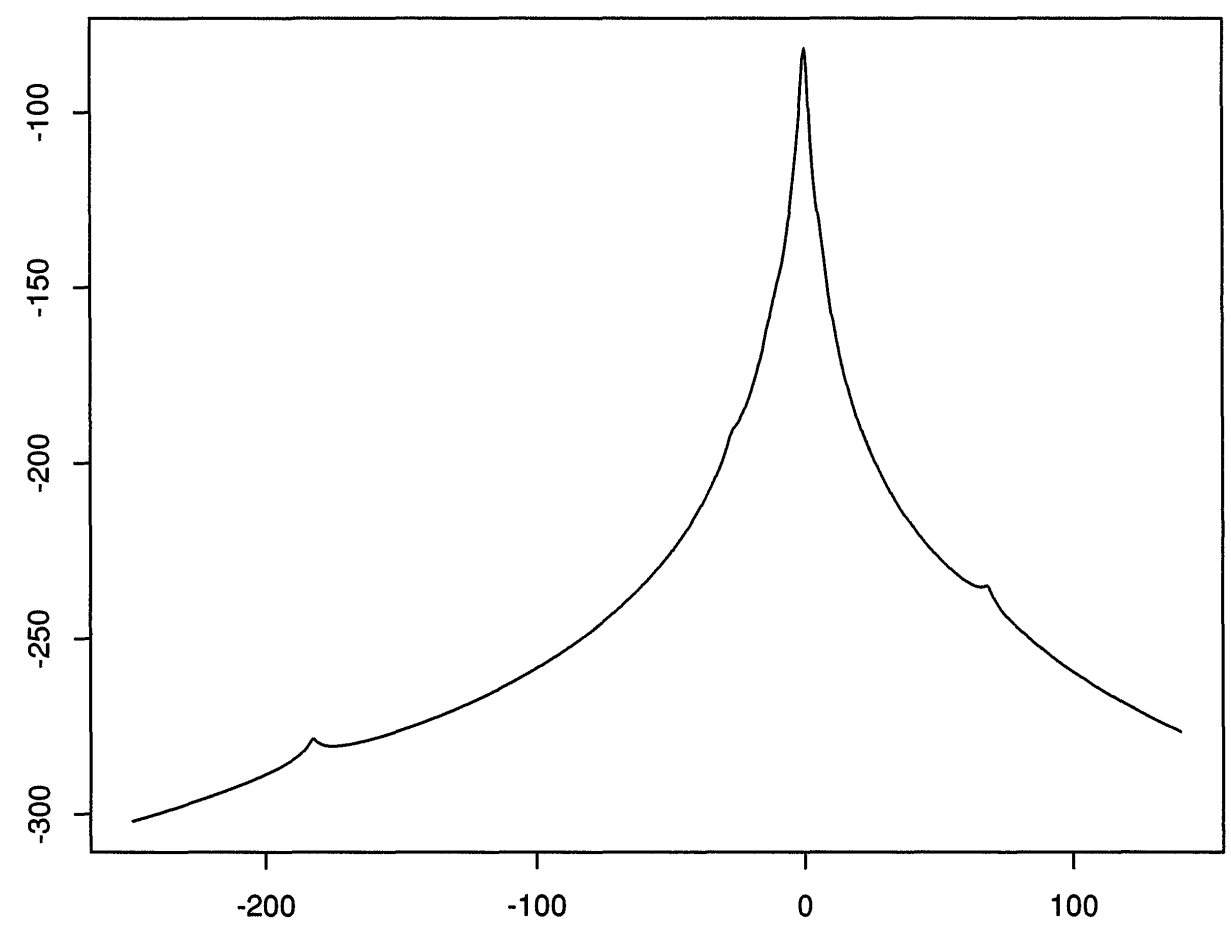
\includegraphics[width=0.72\textwidth]{figures/07-cauchy-log-likelihood.png}
  \caption{Cauchy 位置模型的对数似然函数。图片来自 \cite{vandervaart1998}, p.~74}
  \label{fig:ch7:cauchy-loglik}
\end{figure}

可见有三个局部极大值点，不过全局最大值点是最接近参数真值 0 的，而其它两个则离得很远。关于这个问题，\cite{reeds1985} 曾证明：除了全局最大值的那个点外，其它的``假''局部极大值的个数渐近服从 $\mathrm{Poisson}(1/\pi)$ 分布。


面对 Cauchy 似然方程多根的问题，有一个更加实用的策略，称作\textbf{\emph{单步 MLE}} (One-Step MLE)，其基本思路是利用 Newton 法对一个现有估计进行一步下降：

\begin{enumerate}
\def\labelenumi{\arabic{enumi}.}
\tightlist
\item
  首先选择一个初始的鲁棒估计 $\widehat\theta_0$ ，如样本中位数；
\item
  对 $\widehat\theta_0$ 进行一步 Newton-Raphson 更新： \[ \hat{\theta}_n := \hat{\theta}_0 - \left( \ell_n''(\hat{\theta}_0) \right)^{-1} \ell_n'(\hat{\theta}_0) \]这就是单步 MLE。
\end{enumerate}

单步 MLE 完全不关心似然方程到底有几个根，自然不用在意多根问题。可以证明：单步 MLE 可以改进统计量的效率：虽然 $\widehat\theta_0$ 的渐近方差通常不是最优，但只要它是 $\sqrt n$ -相合的，那么 (在适当正则条件下) $\widehat\theta_n$ 就是渐近有效估计。参考 \cite{shao2003} 一书的 Theorem 4.19。

\end{example}

\subsection{渐近正态性}

MLE 不仅是渐近正态的，也是渐近有效的，即其渐近方差可以达到 C-R 下界 $I^{-1}(\theta)$ 。我们来证明此事。

\begin{theorem}[MLE 的渐近正态性]\label{thm:ch7:mle-asymptotic-normality}

设 $X_1,X_2,\dots,X_n \sim P_{\theta_0}$ i.i.d.，参数空间 $\Theta \subset \mathbb{R}$，存在 $\theta_0$ 的开邻域 $\Theta_0$ 满足：

\begin{enumerate}
\def\labelenumi{\arabic{enumi}.}
\tightlist
\item
  $p_{\theta'}(x) > 0$ 对所有 $x$ 和 $\theta' \in \Theta_0$ 成立；
\item
  $p_\theta(x)$ 在 $\Theta_0$ 内三次可微；
\item
  $p_\theta(x)$ 的三次导数可被控制，即：存在 $M(x) \ge 0$，$\mathbb{E}_{\theta_0}[M(X)] < \infty$，且 $\left|\frac{{\rm d}^3}{{\rm d}\theta^3} \log p_{\theta'}(x)\right| \le M(x)$ 对所有 $\theta' \in \Theta_0$ 成立；
\item
  $p_\theta(x)$ 的积分与一阶、二阶导数可交换，即 $\int \frac{{\rm d}^ip_\theta(x)}{{\rm d}\theta^i} \big|_{\theta=\theta_0} \mathrm{d}\mu(x)=0,\  i=1,2$；
\item
  $0 < I(\theta') < \infty$ 对所有 $\theta' \in \Theta_0$ 成立；
\item
  存在 $\theta_0$ 的 MLE $\widehat\theta_n$ 使得 $\widehat\theta_n\overset P\to \theta$ ，且 $\lim\limits_{n\to\infty}P_{\theta_0}\left(\widehat\theta_n\text{ 是似然方程的唯一解 }\right)=1$ ；
\item
  参数族可识别。
\end{enumerate}

则 \[\sqrt{n} \big(\hat{\theta}_n - \theta_0\big) \overset{\rm d}\longrightarrow \mathcal{N}\left(0, I^{-1}(\theta_0)\right)\]
\end{theorem}

\begin{proof}

仍记 $\ell_n(\theta)$ 是对数似然函数，则 $\hat{\theta}_n$ 满足 $\ell_n'(\hat{\theta}_n) = 0$。在 $\theta_0$ 处作 Taylor 展开：

\begin{equation}
\label{eq:ch7:tag-3}
0 = \ell_n'(\theta_0) + \ell_n''(\theta_0)(\hat{\theta}_n - \theta_0) + \frac{1}{2} \ell_n'''(\tilde{\theta}_n) (\hat{\theta}_n - \theta_0)^2
\end{equation}

其中 $\tilde{\theta}_n$ 位于 $\hat{\theta}_n$ 与 $\theta_0$ 之间。

首先，由弱大数律，

\begin{equation}
\label{eq:ch7:tag-4}
\frac1n\ell_n''(\theta_0) = \frac{1}{n} \sum_{j=1}^n \frac{\partial^2}{\partial \theta^2} \log p_{\theta_0}(X_j) \overset{P}{\longrightarrow} \mathbb{E}_{\theta_0}\left[ \frac{\partial^2}{\partial \theta^2} \log p_{\theta_0}(X) \right] = -I(\theta_0)
\end{equation}

这里期望等于 $-I(\theta_0)$ 用到了条件 (4.)。其次，由条件 (3.)，
\[\frac1n|\ell_n'''(\tilde{\theta}_n)| \le \frac{1}{n} \sum_{j=1}^n M(X_j) \overset{P}{\longrightarrow} \mathbb{E}_{\theta_0}[M(X)] < \infty\]
故 $\tfrac1n\ell_n'''(\tilde{\theta}_n) = O_P(1)$。又因 $\hat{\theta}_n - \theta_0 = o_P(1)$，所以

\begin{equation}
\label{eq:ch7:tag-5}
\frac1n(\hat{\theta}_n - \theta_0)^2 \ell_n'''(\tilde{\theta}_n) = (\hat{\theta}_n - \theta_0)o_P(1)
\end{equation}

我们将式~\eqref{eq:ch7:tag-4}、\eqref{eq:ch7:tag-5} 代入式~\eqref{eq:ch7:tag-3}：\[
0=\frac1n\ell'_n(\theta_0)+\big(-I(\theta)+o_P(1)\big)\big(\widehat\theta_n-\theta_0\big)\]
最后，由经典中心极限定理，\[
\frac1{\sqrt n}\ell_n'(\theta_0) = \frac{1}{\sqrt{n}} \sum_{j=1}^n \frac{\partial}{\partial\theta} \log p_{\theta_0}(X_j) \overset{\rm d}\longrightarrow \mathcal{N}\big(0, I(\theta_0)\big)\]
由 Slutsky 定理直接得出\[ \begin{aligned} \sqrt{n}(\hat{\theta}_n-\theta_0) & =I^{-1}(\theta_{0})\frac1{\sqrt{n}}\ell_{n}^{\prime}(\theta_{0})+o_{P}(1)\\ &\overset{\rm d}\to\mathcal N(0,I^{-1}(\theta_{0})) \end{aligned} \]

\end{proof}

\begin{remark}

\begin{itemize}
\tightlist
\item
  这个定理非常经典，在很多教材中都可以见到，例如 \cite{lehmanncasella1998} 一书的 §6.3 之 Theorem 3.10 (pp.~449-450)。
\item
  在多维情况下，条件 (3.) 需改成 $\Bigl|\frac{\partial^3}{\partial\theta_u\partial\theta_v\partial\theta_w}\log p_\theta(x)\Bigr|\le M(x),\quad u,v,w=1,\dots,k$ ；条件 (5.) 改成 Fisher 信息矩阵 $I(\theta)$ 正定且有限。证明思路与一维类似。
\end{itemize}
\end{remark}

但同时，定理~\ref{thm:ch7:score-root-consistency} 和推论~\ref{cor:ch7:mle-consistency} 的条件也是比较苛刻的：它要求密度二阶或三阶可微、MLE 必须是似然方程的唯一根，等等。这些条件在很多实际模型中不一定满足，或者验证起来很麻烦。在参数空间有良好几何结构的时候，这些条件可以放宽，如下

\begin{theorem*}

设 $X_1,X_2,\dots,X_n \sim P_{\theta_0}$ i.i.d.，$\hat{\theta}_n$ 是基于 $n$ 个 i.i.d. 样本的 MLE。假设：

\begin{itemize}
\tightlist
\item
  $\Theta \subset \mathbb{R}^p$ 为紧致凸集，$\theta_0$ 是 $\Theta$ 的内点；
\item
  所有 $x$ ， $\log p_\theta(x)$ 对 $\theta$ 连续可微，导数满足 $\left|\tfrac{\partial \log p_\theta(x)}{\partial \theta}\right| \le L(x)$，其中函数 $L$ 满足 $\mathbb{E}_\theta[L^2(X_1)] < \infty$；
\item
  参数族可识别。
\end{itemize}

那么 $\widehat\theta_n\overset{P}\to \theta_0$ 。

如果再加上

\begin{itemize}
\tightlist
\item
  $I(\theta)$ 正定且对 $\theta$ 连续。
\end{itemize}

则
\[\sqrt{n}(\hat{\theta}_n - \theta_0) \overset{\rm d}\longrightarrow \mathcal{N}\left(0, I^{-1}(\theta_0)\right)\]

% 最后，关于 MLE 的渐近性质，读者亦可参考笔者基于陈希孺教材整理的笔记，

% \href{https://zhuanlan.zhihu.com/p/1908156011602224244}{数理统计 (15) : 极大似然估计 - 中 - MLE 的相合性}

% \href{https://zhuanlan.zhihu.com/p/1909962170453726655}{数理统计 (16) : 极大似然估计 - 下 - MLE 的渐近正态性}

\end{theorem*}

这个结论来自 \cite{bijma2017} 一书的 Lemma 5.14 和 Theorem 5.9。
\section{基于似然的假设检验}

\subsection{Wald 检验}

基于 MLE 渐近正态性，可以直接构造参数 $\theta$ 的置信域。设 $\Theta\subset\mathbb R^k$ ， $I(\theta)$ 连续，则有
\[\sqrt{n}I^{1/2}(\hat{\theta}_n)(\hat{\theta}_n - \theta) \overset{\rm d}\longrightarrow \mathcal{N}_k(0, \mathbf I_k)\]
从而我们有渐近 $1-\alpha$ 置信域
\[I_\alpha(B_\alpha) = \left\{ \theta : \sqrt{n} I^{-1/2}(\hat{\theta}_n)(\hat{\theta}_n - \theta) \in B_\alpha \right\},\]
其中集合 $B_\alpha \subset \mathbb{R}^k$ 满足 $\mathbb{P}(\mathcal{N}_k(0, \mathbf I_k) \in B_\alpha) = 1-\alpha$。

进一步，对于假设检验 $H_0: \theta = \theta_0$，\textbf{\emph{Wald 检验}} 统计量为
\[W_n := n (\hat{\theta}_n - \theta_0)^\top I(\theta_0) (\hat{\theta}_n - \theta_0) \overset{\rm d}\longrightarrow \chi^2_k\]
拒绝域为 $W_n > \chi^2_k(1-\alpha)$。这个方法非常简单直接，并且不需要一个主观选择的 $B_\alpha$ 。

\subsection{似然比检验}

考虑复合假设
\[
H_0:\theta\in\Theta_0
\qquad\text{对}\qquad
H_1:\theta\in\Theta\setminus\Theta_0.
\]
令 $\hat{\theta}_n$ 为整个参数空间 $\Theta\subset\mathbb R^k$ 上的``全局 MLE''，$\tilde{\theta}_n$ 为 $\Theta_0$ 约束下的``受限 MLE''。定义\textbf{\emph{似然比}} (Likelihood Ratio, LR) 检验统计量为
\[\mathrm{LR}_n :=-2\log\frac{\max_{\theta\in\Theta_0 }\prod_{j=1}^np_{\theta}(X_j)}{\max_{\theta\in\Theta}\prod_{j=1}^np_{\theta}(X_j)}= -2 \log \frac{L_n(\tilde{\theta}_n)}{L_n(\hat{\theta}_n)} = 2 \big( \ell_n(\hat{\theta}_n) - \ell_n(\tilde{\theta}_n) \big)\]
其中 $X_1,\dots,X_n\sim P_\theta$ 是 i.i.d. 样本， $L_n(\theta)$ 和 $\ell_n(\theta)$ 分别是基于这些样本的似然函数和对数似然函数。直观上，若 $H_0$ 成立，则加上约束不应使似然下降太多；若 $\mathrm{LR}_n$ 过大，则倾向于拒绝 $H_0$。似然比、Wald 与 Lagrange 乘子检验的几何关系如图~\ref{fig:ch7:likelihood-tests-geometry} 所示。

\begin{figure}[htbp]
  \centering
  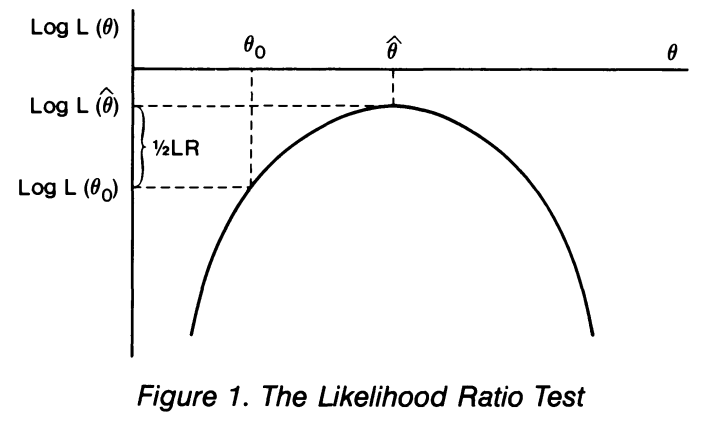
\includegraphics[width=0.78\textwidth]{figures/07-likelihood-tests-geometry.png}
  \caption{似然比、Wald 与 Lagrange 乘子检验的几何关系。图片来自 \cite{buse1982}}
  \label{fig:ch7:likelihood-tests-geometry}
\end{figure}

我们先证明一个辅助引理，

\begin{lemma}[似然比统计量的二次型展开]
\label{lem:ch7:likelihood-ratio-expansion}

设参数空间 $\Theta \subset \mathbb{R}^k$，在定理~\ref{thm:ch7:mle-asymptotic-normality} 的正则条件下，有
\[\begin{aligned} 2(\ell_n(\widehat\theta_n)-\ell_n(\theta_0))&=n(\widehat\theta_n-\theta_0)^\top I(\theta_0)(\widehat\theta_n-\theta_0)+o_P(1)\\ &=\frac1n\ell_n'(\theta_0)^\top I(\theta_0)^{-1}\ell'_n(\theta_0)+o_P(1) \end{aligned}\]
\end{lemma}

\begin{proof}

先证明第一个等式，我们主要利用 $\widehat{\theta}_n$ 是真实参数 $\theta_0$ 的 $\sqrt{n}$‑相合估计，即， $\sqrt n(\widehat\theta_n-\theta_0)=O_P(1)$ 。根据 Taylor 展开：
\[\begin{aligned} 2(\ell_n(\theta_0)-\ell_n(\widehat\theta_n)) &= 2\underbrace{\ell_n'(\widehat\theta_n)^\top (\theta_0-\widehat\theta_n)}_{=0}       +(\theta_0-\widehat\theta_n)^\top \ell_n''(\widehat\theta_n)(\theta_0-\widehat\theta_n) \\ &\quad + \frac13\underbrace{ \sum_{u=1}^k\sum_{v=1}^k\sum_{w=1}^k \frac{\partial^3 \ell_n(\widehat\theta_n)}{\partial\theta_u\partial\theta_v\partial\theta_w}      (\theta_{0u}-\widehat\theta_{nu})(\theta_{0v}-\widehat\theta_{nv})(\theta_{0w}-\widehat\theta_{nw})}_{O_P(n)\cdot O_P(n^{-1/2})\cdot O_P(n^{-1/2})\cdot O_P(n^{-1/2}) = O_P(n^{-1/2}) = o_P(1)} \\      &=(\theta_0-\widehat\theta_n)^\top \ell_n''(\widehat\theta_n)(\theta_0-\widehat\theta_n)+o_P(1)\\      &=-n(\theta_0-\widehat\theta_n)^\top I(\theta_0)(\theta_0-\widehat\theta_n)+o_P(1) \end{aligned}\]
最后一个等号是因为 $\frac1n\ell''(\widehat\theta_n)\overset P\to -I(\theta_0)$ ，从而 $\ell''_n(\theta)=-nI(\theta_0)+o_P(n)$ 。

再证明第二个等式，思路和定理~\ref{thm:ch7:mle-asymptotic-normality} 的证明差不多，由 Taylor 展开 \[ 0=\ell'_n(\widehat\theta_n)=\ell'_n(\theta_0)+\ell_n''(\theta^*)(\widehat\theta_n-\theta_0) \]其中 $\theta^*$ 位于 $\widehat\theta_n$ 和 $\theta_0$ 之间，再利用 $\frac1n\ell''(\theta^*)\overset P\to -I(\theta_0)$ 可知
\[
\sqrt n(\widehat\theta_n-\theta_0)
=I^{-1}(\theta_0)\frac1{\sqrt n}\ell_n'(\theta_0)+o_P(1).
\]
代入第一个等式即可。

\end{proof}

当 $H_0$ 成立时，由于 $\widehat\theta_n-\tilde\theta_n=O_P(n^{-1/2})$ ，因此引理~\ref{lem:ch7:likelihood-ratio-expansion} 的推导也完全成立，我们有 $\mathrm{LR}_n=n(\widehat\theta_n-\widetilde\theta_n)^\top I(\theta_0)(\widehat\theta_n-\widetilde\theta_n)+o_P(1)$ 。这说明 $\mathrm{LR}_n$ 可以（渐近地）看作是对 $\widehat\theta_n$ 和 $\widetilde\theta_n$ 的、用 FI 加权的距离度量。

为研究似然比的渐近分布，我们需要结构化的 $\Theta_0$。假定 $\Theta_0$ 可通过 $r$ 维参数 $a$ 光滑地嵌入原参数空间，这是在说：存在 $g: \mathbb{R}^r \to \mathbb{R}^k$ 使得 $\Theta_0 = \{ g(a) : a \in A \}$，其中 $g$ 二阶连续可微、 $A\subset\mathbb R^r$ ，且真实参数 $\theta_0 = g(a_0)$ ， $a_0$ 为 $A$ 的内点。 $g$ 的可微性保证了 $\Theta_0$ 的局部线性性，这在后面 Wilks 定理的证明中是十分重要的。

这也等同于说，$\Theta_0$ 可由 $k-r$ 个光滑约束 $R(\theta)=0$ 表出，其中 $R:\Theta\to\mathbb R^{k-r}$ ；由于原参数空间是 $k$ 维的，而对 $\Theta_0$ 施加的限制抹除了 $r$ 个自由度，直觉上不难想到，其渐近分布是来自于剩下 $k-r$ 个自由度的。

\begin{theorem}[Wilks 定理]
\label{thm:ch7:wilks}

在上述结构及定理~\ref{thm:ch7:mle-asymptotic-normality} 的正则条件下，当 $H_0$ 成立时，
\[\mathrm{LR}_n \overset{\rm d}\longrightarrow \chi^2_{k-r}\]
\end{theorem}

\begin{proof}

首先，对于全局 MLE，用引理~\ref{lem:ch7:likelihood-ratio-expansion} 可得

\begin{equation}
\label{eq:ch7:tag-6}
2 \big( \ell_n(\hat{\theta}_n) - \ell_n(\theta_0) \big) = \frac{1}{n} \ell'_n(\theta_0)^\top I^{-1}(\theta_0) \ell'_n(\theta_0)  + o_P(1)
\end{equation}

对于受限 MLE $\widetilde{\theta}_n = g(\widehat a_n)$，以 $a$ 为参数，类似可得

\begin{equation}
\label{eq:ch7:tag-7}
2 \big( \ell_n(g(\widehat a_n)) - \ell_n(g(\phi_0)) \big) = \frac{1}{n} \left( \frac{\mathrm{d} \ell_n(g(a_0))}{\mathrm{d} a} \right)^\top \widetilde{I\ }^{-1}\!(a_0) \left( \frac{\mathrm{d} \ell_n(g(a_0))}{\mathrm{d}a} \right) + o_P(1)
\end{equation}

其中 $\widetilde{I\ }\!(a_0) := \mathbb{E}_{\theta_0}\left[ \frac{\partial \log p_{g(a)}(X)}{\partial a} \frac{\partial \log p_{g(a)}(X)}{\partial a}^\top \right]$ 是参数 $a_0$ 的 $r\times r$Fisher 信息矩阵。由求导的链式法则，
\[\begin{aligned}\frac{\mathrm{d}\ell_n(g(a_0))}{\mathrm{d} a} &= g'(a_0)^\top \ell'_n(\theta_0)\\ \widetilde{I\ }\!(a_0) &= g'(a_0)^\top  I(\theta_0)g'(a_0)\end{aligned}\]
这里 $g'(a_0)$ 为 $k \times r$Jacobian 矩阵。

我们将式~\eqref{eq:ch7:tag-6}、式~\eqref{eq:ch7:tag-7} 两式作差，得到
\[\begin{aligned} \mathrm{LR}_n &= 2 (\ell_n(\hat{\theta}_n) - \ell_n(\tilde{\theta}_n)) \\ &= \frac{1}{n} \ell'(\theta_0)^\top \big( I^{-1}(\theta_0) - g'(a_0)(g'(a_0) I(\theta_0) g'(a_0)^\top)^{-1} g'(a_0) ^\top \big) \ell'(\theta_0)+ o_P(1) \end{aligned}\]
令 $Z_n := \frac{1}{\sqrt{n}} I^{-1/2}(\theta_0) \ell'_n(\theta_0)$，由 CLT 有 $Z_n \overset{\rm d}\longrightarrow Z \sim \mathcal{N}_k(0,\mathbf I_k)$。于是
\[\mathrm{LR}_n = Z_n^\top \, M \, Z_n + o_P(1) \overset{\rm d}\longrightarrow Z^\top M Z\]
其中 \[ M := \mathbf I_k - I(\theta_0)^{1/2} g'(a_0) (g'(a_0)^\top I(\theta_0) g'(a_0))^{-1} g'(a_0)^\top I^{1/2}(\theta_0) \]直接验证易知 $M$ 是对称的幂等矩阵（$M^2 = M$），且迹为
\[\begin{aligned} \mathrm{tr}(M) &=\mathrm{tr}(\mathbf I_k) - \mathrm{tr}\big( (g'(a_0)^\top I(\theta_0) g'(a_0))^{-1} g'(a_0)^\top I(\theta_0) g'(a_0)\big)\\ \\ &=k-\mathrm{tr}\Big(\underbrace{\widetilde{I\ }^{-1}\!(a_0)\widetilde{I\ }\!(a_0)}_{\mathbf I_r}  \Big)\\ &=k-r \end{aligned}\]
故 $\mathrm{LR}_n\overset{\rm d}\to\chi^2_{k-r}$ ，如所欲证。

\end{proof}

根据定理~\ref{thm:ch7:wilks}，可以构造近似水平为 $\alpha$ 的接受域 $\{\mathrm{LR}_n\le \chi^2_{k-r}(1-\alpha)\}$，其中 $\chi^2_{k-r}(1-\alpha)$ 代表 $\chi^2$ 分布 $\chi^2_{k-r}$ 的 $1-\alpha$ 分位数。

\begin{remark}

\begin{itemize}
\tightlist
\item
  这个证明也很经典，例如可见 \cite{serfling1980} 的 4.4 节、\cite{shao2003} 一书的 Theorem 6.5 或者 \cite{chenxiru2009} 一书的定理 6.1 等。
\item
  在复合假设下，我们也可以把之前简单假设下的 Wald 检验进行修改，由 Delta 方法： \[ \sqrt nR(\widehat\theta_n)\overset{\rm d }\longrightarrow\mathcal N_{k-r}\big(0,R'(\theta_0)I^{-1}(\theta_0)R'(\theta_0)^\top\big) \]可以得到如下 \emph{Wald 检验}统计量： \[ W_n:=nR(\widehat\theta_n)^\top\big(R'(\widehat\theta_n)I^{-1}(\widehat\theta_n)R'(\widehat\theta_n)^\top\big)^{-1}R(\widehat\theta_n) \]此外还有 \emph{Rao's Score 检验}，其形式来自引理~\ref{lem:ch7:likelihood-ratio-expansion} 的第二个等式，我们用\emph{插入原则} (plug-in principle)，对 $I(\theta_0)$ 用 $I(\widetilde\theta_n)$ 估计之，对 $\ell'(\theta_0)$ 用 $\ell'(\widetilde\theta_n)$ 估计之，即可得到如下检验统计量
  \[
  R_n:=\frac1n\ell'_n(\widetilde\theta_n)^\top
  I^{-1}(\widetilde\theta_n)\ell'_n(\widetilde\theta_n).
  \]
  读者可以验证：似然比检验、Wald 检验、Rao's Score 检验，三者在原假设下是渐近等价的。相比于似然比检验统计量要算两个 MLE，Wald 检验只看全参数空间下的 MLE，而 Rao's Score 检验只看受限参数空间的 MLE，因而二者在计算上更加简单。
\item
  一个例子是存在讨厌参数 (Nuisance Parameter) 的假设检验问题。设参数分为 $\theta = (\beta, \gamma)$，其中 $\beta$ 是我们感兴趣的参数，$\gamma$ 是讨厌参数。我们关心检验
  \[
  H_0:\beta=\beta_0
  \qquad\text{对}\qquad
  H_1:\beta\ne\beta_0.
  \]
  设全参数空间的 MLE 为 $\hat\theta_n = (\hat\beta_n, \hat\gamma_n)$，而受限于 $H_0$ 的 MLE 为 $\tilde\gamma_n = \operatorname*{\arg\sup}\limits_{(\beta_0,\gamma)\in\Theta} \ell_n(\beta_0,\gamma)$ ，后者也被称作是 $\beta_0$ 的轮廓似然 (Profile Likelihood
  % 例如可见 \url{https://www.zhihu.com/question/310585422}
  )。在正则条件满足时，有似然比统计量\[ \mathrm{LR}_n(\beta_0) = 2\bigl( \ell_n(\hat\beta_n, \hat\gamma_n) - \ell_n(\beta_0, \tilde\gamma_n) \bigr) \]设 $\Theta = \Theta_\beta \oplus \Theta_\gamma$ （ $\beta,\gamma$ 的参数空间正交），且 $\dim\Theta=k$ 、 $\dim\Theta_\gamma = r$。那么根据定理~\ref{thm:ch7:wilks}，在 $H_0$ 下\[ LR_n(\beta_0) \overset{\rm d}\longrightarrow \chi^2_{k-r} \]从而，我们有近似的接受域 $\{\beta:\mathrm{LR}_n(\beta)\le \chi^2_{k-r}(1-\alpha)\}$ 。
\end{itemize}
\end{remark}

\begin{example}[Wilks 定理的反例]
如果正则条件不满足，则定理~\ref{thm:ch7:wilks} 的极限分布可能不适用。如，设 $X_i \sim \mathcal U(0,\theta)$，由于参数位于密度支撑集的边界，这违背了定理~\ref{thm:ch7:mle-asymptotic-normality} 的第 (1.) 条。我们想检验
\[
H_0: \theta = \theta_0\quad \iff\quad H_1:\theta\ne \theta_0,
\]
其中 $\theta_0>0$ ；由于 MLE 为 $X_{(n)}$，且原假设下的似然函数为 $L_n(\theta_0)=\theta_0^{-n}$ ，则似然比统计量为
\[
\mathrm{LR}_n = -2n \log\frac{X_{(n)}}{\theta_0}\quad \text{ 当 }X_{(n)}\le \theta_0.
\]

当原假设成立时，周知 \[ Y_n:=n\frac{\theta_0-X_{(n)}}{\theta_0}\overset{\rm d}\to\mathrm{Exp}(1)\overset{\rm d}=\frac12\chi_2^2 \]从而 \[ \mathrm{LR}_n=-2n\log\left(1-\frac{Y_n}n\right)=2Y_n+o_P(1)\overset{\rm d}\to \chi_2^2 \]极限分布为 $\chi^2_2$，自由度是不符合定理~\ref{thm:ch7:wilks} 的。


\end{example}

\subsection{Bartlett 校正}

虽然 Wilks 定理给出了 $\mathrm{LR}_n$ 的极限分布，但在有限样本下，其分布毕竟还是与 $\chi^2_{k-r}$ 有差距，例如相比于 $\mathbb{E}[\chi^2_{k-r}]=k-r$ ， $\mathbb{E}[\mathrm{LR}_n]$ 往往偏大。Bartlett 在 1937 年提出了 ``\textbf{\emph{Bartlett 较正}} (Bartlett correction)''，其出发点就是希望在有限样本下校正此类偏差，从而改进似然比检验。其核心观察在于， $\mathrm{LR}_n$ 的期望可以展开为
\[
\mathbb{E}[\mathrm{LR}_n] = (k-r) + \frac{b_1}{n} + o(n^{-1}) = (k-r)\left(1 + \frac{b}{n} + o(n^{-1})\right).
\]

其中 $b$ 或 $1 + \frac{b}{n}$ 被称为 \textbf{\emph{Bartlett 因子}} (Bartlett factor)。这样一来， $\tfrac{\mathrm{LR}_n}{1+b/n}$ 就十分符合我们的要求：它的期望与目标极限分布 $\chi^2_{k-r}$ 之间仅相差 $o(n^{-1})$ 。

当然， $b$ 本身取决于 $\theta_0$ ，也是未知的；若能得到 $b$ 的一个相合估计 $\widehat{b}_n \stackrel{P}\to b$，则可以定义 Bartlett 校正的似然比统计量 
$$\mathrm{LR}_{n, bc} := \frac{\mathrm{LR}_n}{1 + \hat{b}_n / n}$$
由 Slutsky 定理，其仍满足 $\mathrm{LR}_{n, bc}\overset{\rm d}\to \chi^2_{k-r}$ 。

Bartlett 校正 $\mathrm{LR}_{n, bc}$ 真的能比 $\mathrm{LR}_{n}$ 取得更好的近似吗？这里更进一步地探讨一下：首先 Wilks 定理告诉我们，在原假设下， 

$$\lim_{n \to \infty} P(\mathrm{LR}_n \le x) = P(\chi^2_{k-r} \le x)$$
即逼近误差为 $o(1)$；若进一步使用 Edgeworth 展开（需要更强的矩条件和尾部性质，如 \emph{Cramér 条件}，见第~\ref{ch:characteristic-functions}~章），实际上可以证明 \cite{hayakawa1977,chandraghosh1979}：

$$P(\mathrm{LR}_n \le x) = P(\chi^2_{k-r} \le x) + O(n^{-1})$$

对于检验简单原假设 $H_0: \theta = \theta_0$ 的情形， $\mathrm{LR}_n\overset{\rm d}\to\chi_k^2$ ，一般有\[
\mathbb{E}[\mathrm{LR}_n(\theta_0) ] = k\left(1+\frac\beta n\right)+O(n^{-2})\]
即期望仅在首阶与 $\chi^2_k$ 的均值 $k$ 一致。更精细地 \cite{barndorffnielsencox1984,barndorffnielsenhall1988}：\[
P(\mathrm{LR}_n(\theta_0) \le x) = P(\chi^2_k \le x) - \beta x g_k(x) n^{-1} + O(n^{-2})\]
其中 $g_k$ 是 $\chi^2_k$ 的密度函数；此时如果采用 Bartlett 校正，那么\[
P\left( \frac{\mathrm{LR}_n}{1 + \beta n^{-1}} \le x \right) = P( \chi^2_{k} \le x ) + O(n^{-2})\]
且当 $\widehat\beta_n$ 是 $\beta$ 的 $\sqrt n$ -相合估计时，
\[
P\left( \frac{\mathrm{LR}_n}{1 + \hat{\beta} n^{-1}} \le x \right) = P( \chi^2_{k} \le x ) + O(n^{-3/2}).
\]

这从理论上表明，Bartlett 校正确实可以将似然比统计量分布逼近精度提高。
